\documentclass[tikz, border=8pt]{standalone}
\usepackage{amsmath}

\begin{document}
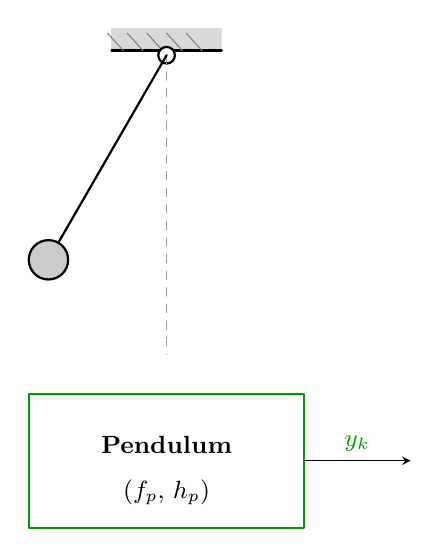
\begin{tikzpicture}[line cap=round, line join=round, >=stealth, font=\small]

  % ── Physical pendulum ────────────────────────────────────────────────────────

  % Wall mount
  \fill[black!15] (-0.7, 0.06) rectangle (0.7, 0.35);
  \draw[thick] (-0.7, 0.06) -- (0.7, 0.06);
  \foreach \xi in {-0.55,-0.30,-0.05,0.20,0.45}
    \draw[thin, black!50] (\xi, 0.06) -- ++(-0.20, 0.22);

  % Pivot
  \filldraw[fill=white, draw=black, thick] (0,0) circle (3pt);

  % Dashed vertical
  \draw[dashed, black!40, thin] (0,0) -- (0,-3.8);

  % Rod
  \draw[thick] (0,0) -- (-1.5, -2.598);

  % Bob
  \filldraw[fill=black!20, draw=black, thick] (-1.5, -2.598) circle (0.25);

  % ── Block ────────────────────────────────────────────────────────────────────

  \draw[thick, green!60!black] (-1.75, -4.3) rectangle (1.75, -6.0);
  \node[font=\small\bfseries\upshape] at (0, -4.95) {Pendulum};
  \node[font=\small\itshape]          at (0, -5.55) {$(f_p,\,h_p)$};

  % Output arrow
  \draw[->] (1.75, -5.15) -- (3.1, -5.15);
  \node[above, font=\small\itshape, green!60!black] at (2.42, -5.15) {$y_k$};

\end{tikzpicture}
\end{document}
